% !TEX root = morphkasten.tex

\section{Lenkung}


%############## Trapez
\subsection{Trapez}

\begin{figure} [hbp]
	\centering
	\begin{subfigure}[b]{0.4\textwidth}
		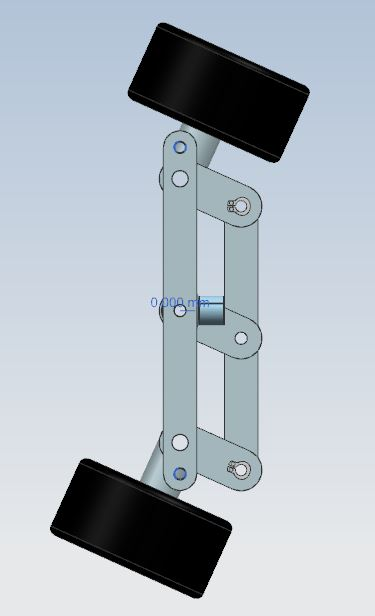
\includegraphics[width=\textwidth]{fig/Trapezlenkung3.JPG}
		\caption{1.Situation: CAD-Modell}
	\end{subfigure}
	\hfill
	\begin{subfigure}[b]{0.36\textwidth}
		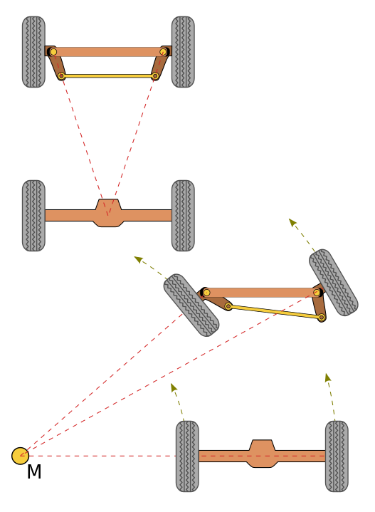
\includegraphics[width=\textwidth]{fig/Lenktrapez.png}
		\caption{2. Situation: Trapezlenkung
		(Quelle: http://www.portmanns.ch/Repetition/Fahrwerk/Lenkungsarten.pdf)}
\end{subfigure}
	\caption{Trapezlenkung}\label{fig:animals}
\end{figure}

\begin{table}[h]
\begin{tabular}{p{0.5\textwidth} | p{0.5\textwidth}}


 \textbf{Vorteile} & \textbf{Nachteile} \\ \hline
	 
\begin{itemize}
\item Konventionelle oft verwendete Lenkung für PWS
\item Berechnungen für Lenkgeometrie im Internet
\item Viele Reale Beispiele als Vorlag
\item ...
\end{itemize}

 
 &
 
\begin{itemize}
\item Herstellung relativ aufwändig
\item Kamera ist in der Kurve nicht 90 Grad zur Strecke
\item Nachteil 3
\item 
\end{itemize}

\end{tabular}
\end{table}

\begin{table}[h]
\begin{tabular}{p{0.5\textwidth}p{0.5\textwidth}}


 \textbf{Risiken} & \\ \hline
	 
\begin{itemize}
\item Risiko 1
\item Risiko 2
\end{itemize}
&
\begin{itemize}
\item Risiko 3
\item ...
\end{itemize}

 
\end{tabular}
\end{table}

\pagebreak


%############## Raupen
\subsection{Raupen}
Im Kapitel 1.1 wurden die Variante Raupen bereits beschrieben.


%############## 2 Räder mit 2 Motoren
\subsection{2 Räder mit 2 Motoren}

Grafik

\begin{table}[h]
\begin{tabular}{p{0.5\textwidth} | p{0.5\textwidth}}


 \textbf{Vorteile} & \textbf{Nachteile} \\ \hline
	 
\begin{itemize}
\item Vorteil 1
\item Vorteil 2
\item Vorteil 3
\item ...
\end{itemize}

 
 &
 
\begin{itemize}
\item Nachteil 1
\item Nachteil 2
\item Nachteil 3
\item ...
\end{itemize}

\end{tabular}
\end{table}

\begin{table}[h]
\begin{tabular}{p{0.5\textwidth}p{0.5\textwidth}}


 \textbf{Risiken} & \\ \hline
	 
\begin{itemize}
\item Risiko 1
\item Risiko 2
\end{itemize}
&
\begin{itemize}
\item Risiko 3
\item ...
\end{itemize}

 
\end{tabular}
\end{table}

\pagebreak